\chapter{Background}\
\label{chap:background}
This section tackles the fundamental principles and groundwork of the theory encompassing concepts, terminology, and methodologies related to search engines as applied within this thesis.

\section{The nature of the web}
The web we know today, Web 2.0, is known as "the participative social web" and is massive, and its rate of change is enormous due to its highly dynamic content. Due to this big sample space, finding the relevant pages or documents from the web isn't easy. To overcome this issue, there are two main approaches to sampling: 
Vertical sampling: Focus only on the pages that are restricted by the domain name. This can be done in different levels. For example, one can restrict the crawling process based on the country, such as .de, .ly, uk. When vertical sampling is done at the second level, it limits the crawling to domains (e.g. stanford.edu) [3].
Horizontal sampling: In this approach, it is important to know the most visited pages and domains to keep crawling from them, giving them more priority than others. This can be done by collecting data logs from the ISP or utilising a web crawler to estimate the page's popularity [3]. 


\section{History}
\numberwithin{equation}{chapter}

The World Wide Web is an unlimited space to share provide and share information. Those information can have different format and cover different doamins. The use case of the web is only limtied by the developers imagination. This is benifital as the Web keept evolving rapidaly form Web 1.0 to Web 2.0 to Web 3.0. Web 1.0 used static pages to serve information, those information were moslty news, blogs and personal langing pages. Some refre to the Web 1.0 as "the read-only web". Although Web 1.0 was massive however most content were created was by deverlopers or at least users who knew basics of the HTML and CSS, moreover by that time content were only static they did not depen on fancy JavaScript libraries and frameworks like Angular and React, this made it limited to some use cases only. Fast forward, pages become more dynamic after using sessions, databases and clint rendering schemas. Those changes made the Web focused not only reading and gathering information by gave the power to more audiounce who did not know any programming or coding to participate and interact with the Web via browsers. Social media, e-commerce and trading stocks platforms was one of the reasons made the internet buble inflate, Use cases where unlimited as useres could create and deploy their own websites by using simple tools as Content Manament System CMS. This made Web 2.0 known as "the participative social web".

To optimize the allocation of crawler resources, estimating the page's freshness must be considered. This prevents outdated pages from remaining unrefreshed for prolonged periods or where lesser-significant pages are needlessly recrawled despite unchanged content.


It can be understood intuitively that the likelihood of a copy of page p being up-to-date at time t, denoted as up(t), declines over time when the page is not revisited.

\begin{equation}
u_p(t) \propto e^{-\lambda_pt}
\label{eq:depth}
\end{equation}

The parameter λp signifies the rate of modifications occurring on page p, and its estimation can be deduced from past observations, mainly when the web server indicates the page's last modification date during visits. Cho and Garcia-Molina derived this estimation technique for λp [8].

\begin{equation}
\lambda_p \approx \frac{(X_p-1) - \frac{X_p}{N_p\log(1-X_p/N_p)}}{S_pT}
\label{eq:depth}
\end{equation}

\begin{itemize}
  \item Np number of visits to p.  
  \item Sp time since the first visit to p.
\item Xp number of times the server has informed that the page has changed.
\item Tp total time with no modification, according to the server, summed over all the visits.
\end{itemize}

Note that some pages do not include the last-modified time stamp, and in this case, one can estimate this manually by comparing the
downloaded copies at two different times and using the following equation. Where Xp now will be the number of times a modification is detected.

\begin{equation}
\lambda_p \approx \frac{-N_p\log(1-X_p/N_p)}{S_p}
\label{eq:depth}
\end{equation}

\section{Web Search Engine}
Web Search Engine is software that collects information from the web and indexes them efficiently to optimize the searching process by the user. Users enter their queries to ask for information. The engine performs queries, looks up the pre-built organized index, and returns relevant results. The returned result is presented by Search Engine Results Pages as known as SERPs. The result is then ranked based on predefined criteria. 

Web search engines use web crawlers or spiders to collect and harvest the internet jumping from one page to another. Each page can contain several links. The crawler's task is to find the links, visit them, and harvest them. Followed by crawlers, indexing is the next process where information is organized and optimized for search. 

\begin{figure}[h]	
     \centering
         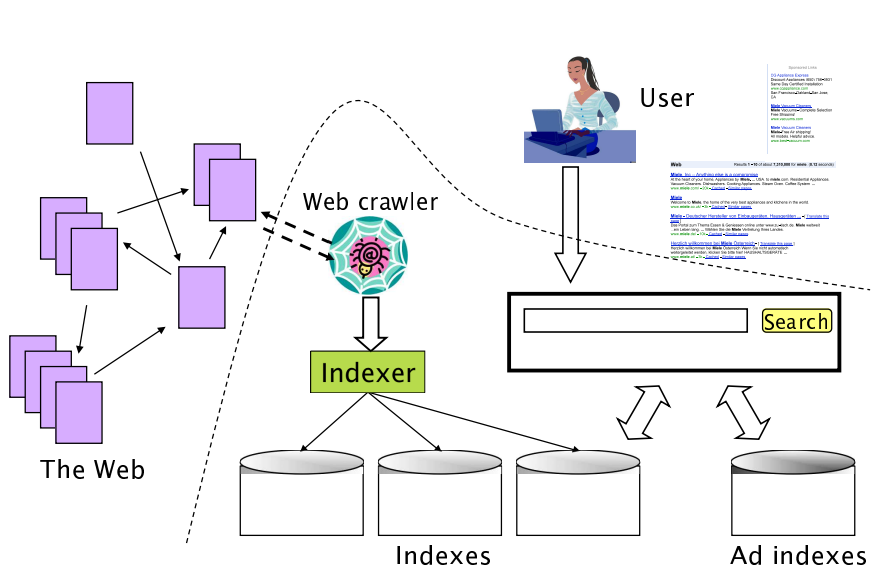
\includegraphics[width=10cm]{images/engine_components.png}
\end{figure}

\subsection{Requierments and Features}
Search engines, regardless of their imp[lmentation and design there, are some features and requirements that make a good one; following is a list of the most fundamentals features:  

\begin{itemize}
  \item Web Crawling and Indexing: Each search engine needs two main big components, Crawler and Indexer. The Crawler is the component responsible for collecting pages and downloading them from the web. An indexer is used to create an index to facilitate efficient searching.
  \item Ranking and Relevancy: The algorithm determines the order in which search results are presented to users based on relevance.
  \item User Interface: The user interface where users enter their search queries and view results.
  \item Scalability and Performance: Distributed Architecture: A distributed system helps handle the vast amount of data and traffic. This needs a Load balancer to distribute the cralwing tasks betrween the nodes and threads. 
  \item Data Storage and Management: A robust database system is necessary for storing indexed data and metadata.
\end{itemize}

\section{Cralwer}
Web crawler or spider is a software which gathers pages information from the web, to prived the necessary data to the Indexer to build a search engine. The essential role of crawlers is to effectively and reliably collect as much information from the web. This thesis invests more time on this component than the Indexer as it serves as the bottleneck to the Search engine performance. 

\subsection{Cralwer Specifications}
Crawlers can have a wide vireity of features and specifications, however some are necessary to include and others are vital to have a reliable useable one. More information can be found in the book [9] 

\begin{itemize}
\item Robustness: Web crawlers can be fragile and easy to break; this is due to the nature of the dynamic contents on the web and the internet connection. Web crawlers must identify those edge cases and obstacles and tackle them.  

\item Politeness: The implementation of the crawler can be unintentionally Mellitus and dangerous if not designed correctly. A Denial of service DoS and a Distributed Denial of service DDoS attacks can occur due to a bad crawler implementation. Hence crawlers must respect websites policies and avoid breaking up web services and loading the servers.

\item Distributed: For optimal efficiency, the crawler should possess the capacity to operate in a distributed manner across numerous machines.

\item Scalable: The crawler's design should enable the expansion of the crawl rate by seamlessly integrating additional machines and bandwidth.

\item Performance and efficiency: The crawling system should adeptly utilize various system resources, including processor capacity, storage capabilities, and network bandwidth.

\item Quality: The crawler should be biased towards
fetching "useful" pages first.

\item Freshness: Acquiring recent versions of previously accessed pages. This is particularly relevant for search engine crawlers, ensuring the search index remains updated.

\item Extensible: Crawler design should possess extensibility across numerous dimensions, facilitating adaptation to novel data formats, emerging fetch protocols, and similar challenges. This necessitates a modular architecture that accommodates expansion.
\end{itemize}

\subsection{Crawler architecture}

The simple crawler architecture is made of the following fundamental modules, as shown in the following Figure. Fetch module that communicates with the internet and collects the pages passed by the URL Frontier module using HTTP requests from the URLs. URL frontier module contains a list of the URLs that need to be fetched by the Fetch module. Parsing module that takes the page content found by the fetch module and parses the page content to find the following links to be passed to the URL frontier and also to parse any value needed from the page, like text and images. Duplication filter that is used to exclude seen URLs. The DNS resolution module is responsible for identifying the web server from which to retrieve the page indicated by a given URL [9]. 

\begin{figure}[h]	
     \centering
     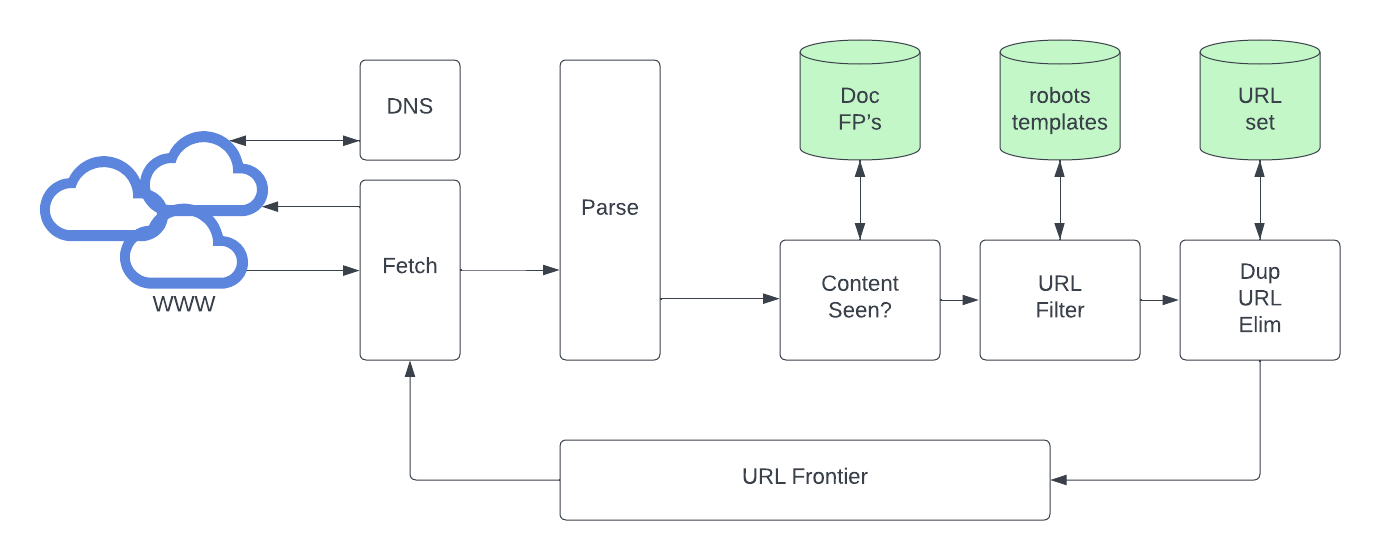
\includegraphics[width=10cm]{images/crawler_architecture.png}
     \caption{The basic crawler architecture.}
     \label{fig:google-arch}
\end{figure}

The first step is to add a seed URL to the URL frontier. This URL works as a starting point for crawling. The crawler then fetches the page corresponding to the seed URL and stores it to be parsed by the parser. Subsequently, the page undergoes parsing to extract both its textual content and embedded links. The content will be used by the indexer component in the search engine. Moreover, each identified link by the parser module is subjected to a set of evaluations to determine its eligibility for addition to the URL frontier.

After finding the future links and content by the parser, filtering both found links and content is needed. The first step is to check if the page content has already been seen; this can be done by checking the page content fingerprint. The most straightforward method is to use a checksum (stored in the Doc FP's). The next filter is to exclude the parsed new URLs. The URL filter will run some tests to exclude unwanted URLs. This can be some URLs out of the country target, like .de, or some restricted URLs that should not be visited by the crawler. Excluded URLs list can be added manually to the filter. However, there are more rules written by the domain admins that should be followed. Those rules can be found under a standard text file named Robots Exclusion Protocol (robots.txt). 

"robots.txt" acts as the selected filename for implementing the Robots Exclusion Protocol, which is a widely adopted standard employed by websites to signal to web crawlers and other web robots the specific sections of the website that are permissible for them to access [10]. The "robots.txt" can be fetched at the starting point of crawling and can be cached through the whole crawling process, as it can be assumed it will not change during the crawling process. This assumption is still better than making an HTTP request to get the robots.txt file for each URL that needs to be fetched, as this will duplicate the number of requests and reduce the crawler efficiency and also load the server with unwanted requests. Including the robots.txt in the crawling, process should be mandatory as this will serve the point about politeness mentioned in the Crawler specifications section. 

\subsection{Web Crawler Types}
It is essential to understand that although all web crawlers' main goal is to crawl pages from the internet, however, there are different types and categories that some crawlers fall to. The first category is  Universal or Broad crawler. This category of web crawlers doesn't confine itself to webpages of a specific topic or domain; instead, they continuously traverse links without limitations, collecting all encountered webpages. The most significant search engines use this type of crawler, such as Google and Bing, this is understandable as these search engines' main aim is to make the entire web searchable, and they try to fetch all kinds of pages and contents. The second category is called Preferential crawler (Focused crawler). Focused crawlers target specific topics, themes, or domains. They are designed to gather information from a particular niche or subject area, providing specialized search results. In this thesis, a Focused crawler has been implemented and used. The last category is Hidden Web crawlers (Deep Web Crawlers). Deep web crawlers target databases and content hidden behind web forms. They can interact with online databases and retrieve information that general search engines might miss [11].

\subsection{Challenges and issues}
Researchers encounter a variety of challenges when working with different crawlers implementation. A compilation of these challenges is presented below.


\begin{itemize}
\item The scale of the web: The web is vast and virtually infinite, so crawlers must prioritize which pages to crawl and which to skip to use resources efficiently.

\item Content Changes: Webpages can change frequently, requiring crawlers to revisit and reindex content to ensure freshness and accuracy.

\item Blocking and IP Bans: Some websites may block or ban crawlers' IP addresses if they perceive them as causing too much traffic or disruption. Crawlers need to manage IP addresses to avoid being blocked.

\item Nonuniform structures: The Web is dynamic
and uses inconsistent data structures, as there is
no universal norm to build a website. Due to lack of uniformity, collecting data becomes difficult. The problem is amplified when crawler has to deal with semistructured and unstructured data.

\item Error handling: Crawlers may encounter broken links, leading to errors and incomplete indexing. Handling broken links requires additional processing. Moreover, the internet connection may disconnect, and the crawler may stop crawling. 

\item Crawlers traps: Some websites intentionally create spider/crawlers traps to make crawlers go into an infinite loop or redirect them in different directions. Calendar Traps and Infinite URL Parameters are examples of spider traps.

\item Politeness and Ethical Concerns: Crawlers must be programmed to be polite and respectful to websites' server resources. Aggressive crawling can overload servers, leading to ethical concerns and potential website blocking. This might be simple, but the main challenge is that each domain uses different Firewall settings. One server might allow the crawler to make five requests per second; the other will block the crawler. There are no hardcoded rules to follow; however, following the robots.txt file might help improve the  Politeness of the crawler.
\end{itemize}


\\


\section{Indexing}
In a search engine, an indexer is a component responsible for analyzing and organizing the content of web pages or documents in order to create an index, which is a structured database that enables efficient and fast retrieval of relevant information during search queries.
When a search engine's crawler or web spider gathers data from websites, the indexer processes this data by breaking down the content into smaller units like words, phrases, and metadata. It then associates these units with the URLs or documents they came from. This organized information is stored in the index, which serves as a map or reference for the search engine to quickly locate and present relevant results when a user makes a search query.
The indexer plays a crucial role in improving the speed and accuracy of search results because it precomputes and structures the data in a way that enables the search engine to match queries with indexed content more efficiently. Although supporintg indexing is fundemantal in this thesis however it will be given less attention than the crawling component. 

\subsection{Inverted index}
Crawlers collect information from the web and prepare them to be searched. However, looking up each term with brute forcing is a performance issue and is impossible. Hence inverted index data structure is used. 
An inverted index or inverted file is a data structure used in information retrieval systems, particularly in search engines, to store and efficiently retrieve information about the occurrences of terms (words or phrases) within a collection of documents. It is called "inverted" because it inverts the relationship between terms and documents compared to traditional databases, where documents are associated with their content.
In an inverted index, each unique term in the collection of documents is treated as a key, and the value associated with each term is a list of references to the documents where that term appears. This list of references allows for rapid access to all the documents containing a specific term.

Creating an Inverted index requires the next steps. The first step is to collect the documents to be indexed. In the context of this thesis, the documents referred to the content inside the crawled pages. The second step is to tokenize the text, turning each document into a list of words known as tokens. The last step is to create a dictionary that maps each term with a list of the ids of the documents that occurred. The tokenized terms are called dictionaries, and the list of ids is called postings. 

\begin{figure}[h]	
     \centering
     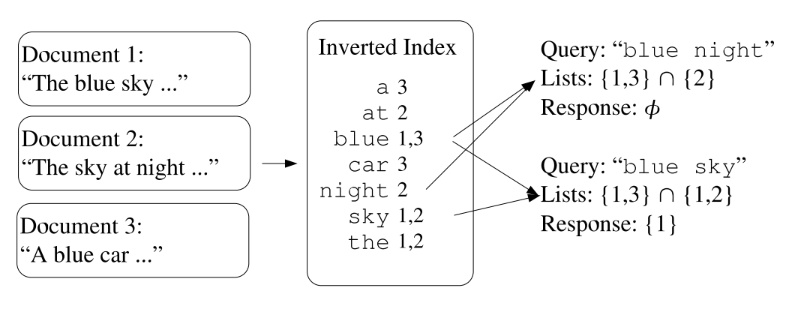
\includegraphics[width=10cm]{images/inverted_index.png}
     \caption{
An illustration of an inverted index featuring three documents. All tokens are included in this example, and the sole text normalization applied is converting all tokens to lowercase. Queries that involve multiple keywords are resolved using set operations. [3]}
     \label{fig:google-arch}
\end{figure}

\section{Ranking}
As discussed indexing process prepares a map that can be looked up to find relevant terms that match the search query; however, one needs to rank the returned result based on relevance. For example, a user searching "for what is Freiburg?" will be expecting a result about Freiburg and not to return all documents that contain tokens like "what" and "is". So how can we find the relevant documents? There are many algorithms for document ranking. However, in this thesis, BM25 will be adopted. 

\begin{equation}
BM25\_score = tf^*.\log_2(\frac{N}{df})
\label{eq:depth}
\end{equation}
\begin{equation}
tf^* = \frac{tf.(k+1)}{k.\alpha+tf}
\label{eq:depth}
\end{equation}
\begin{equation}
\alpha = \frac{1-b+b.DL}{AVDL}
\label{eq:depth}
\end{equation}

\textit{N} = Total number of docuemnts, \textit{tf} = term frequency, the number of times a word occurs in a document, \textit{df} = docuemnt frequency, The number of documents containing a particular word, \textit{DL} = document length, \textit{AVDL} =
average document length (measured in number of words)
Standard setting for BM25: \textit{k} = 1.75 and \textit{b} = 0.75
